\chapter{Development Plan}
\label{chap:Chapter5}
%-------------------------------------------------------------------------------%
\section{Research Approach}
To achieve the desired objectives and system requirements, the development approach will be composed of three phases: Dissertation Development, System Development, and Implementation.

During the first part of dissertation development, it will be analyzed the problems with fixed-pitch propeller systems, described in the previous chapters, in \glspl{uav} to be able to find the best approach to solve the issue at hand, to define the new system requirements, determine the objectives of the proposed solution and to design the system architecture.
And, to gain a better understanding of the present status of the subject, a study of the literature related to the problem, will be conducted.
In this phase, it will be also written all the steps and considerations taken during the development and implementation of the solution and an analysis of the results obtained.

As we go on to the System Development phase, there will be a detailed procurement to find the most adequate components, according to the system architecture and requirements, since it is necessary to design and manufacture \glspl{PCB} for the final prototype.
In this phase, the system flow charts, shown in the appendix, will be modeled and validated using model checker tools like NuSMV.
This step will increase the confidence in the chosen firmware and validate the expected behavior of the system.

In the implementation phase, the Main and Secondary Devices will be soldered and assembled, to, later on, perform, bench and ground tests, and evaluate the developed system in comparison to predetermined goals and requirements.
By documenting and analyzing the results it will be possible to make any necessary refinements to enhance performance.

%-------------------------------------------------------------------------------%

\section{Evaluation}
In order to evaluate the system's performance, in comparison to the requirements, the analyses will be divided into three categories.

In the Communication category, it will be analyzed the stability and the latency of the chosen communication technology.

Another category is the Pitch Angle Control in which the precision and stability of the control over the pitch angle will be evaluated.
It will also be analyzed if the system has a quick response to changes in flight phase and Maneuver, a quick response in error scenarios and if the fail-safe mechanism can set a fixed pitch angle.

The last category to be evaluated is the Firmware.
In this category, the model of the system flow will be validated with mathematical tools as explained before.

This way, the system will be evaluated in each subsystem and as a whole.

%-------------------------------------------------------------------------------%

\section{Timeline}
In the Gantt chart (figure \ref{fig:gantt}) all phases, described previously in the Research Approach section, were added together with multiple tasks and subtasks each with a given duration and dependencies.

The first task started is the Research Plan, part of the Dissertation Development phase, and will be the starting point of future work.
All the other tasks, in this phase, will be done in parallel until the end of the dissertation.

Next will be the System Development phase where hardware and firmware tasks will be made.
These tasks will start in mid-January 2024 and end in early April 2024.

The last tasks will be from the Implementation phase with tests, evaluations and refinement tasks.
They will be carried out from mid-March 2024 to mid-July 2024.

\begin{figure}[H]
    \centering
    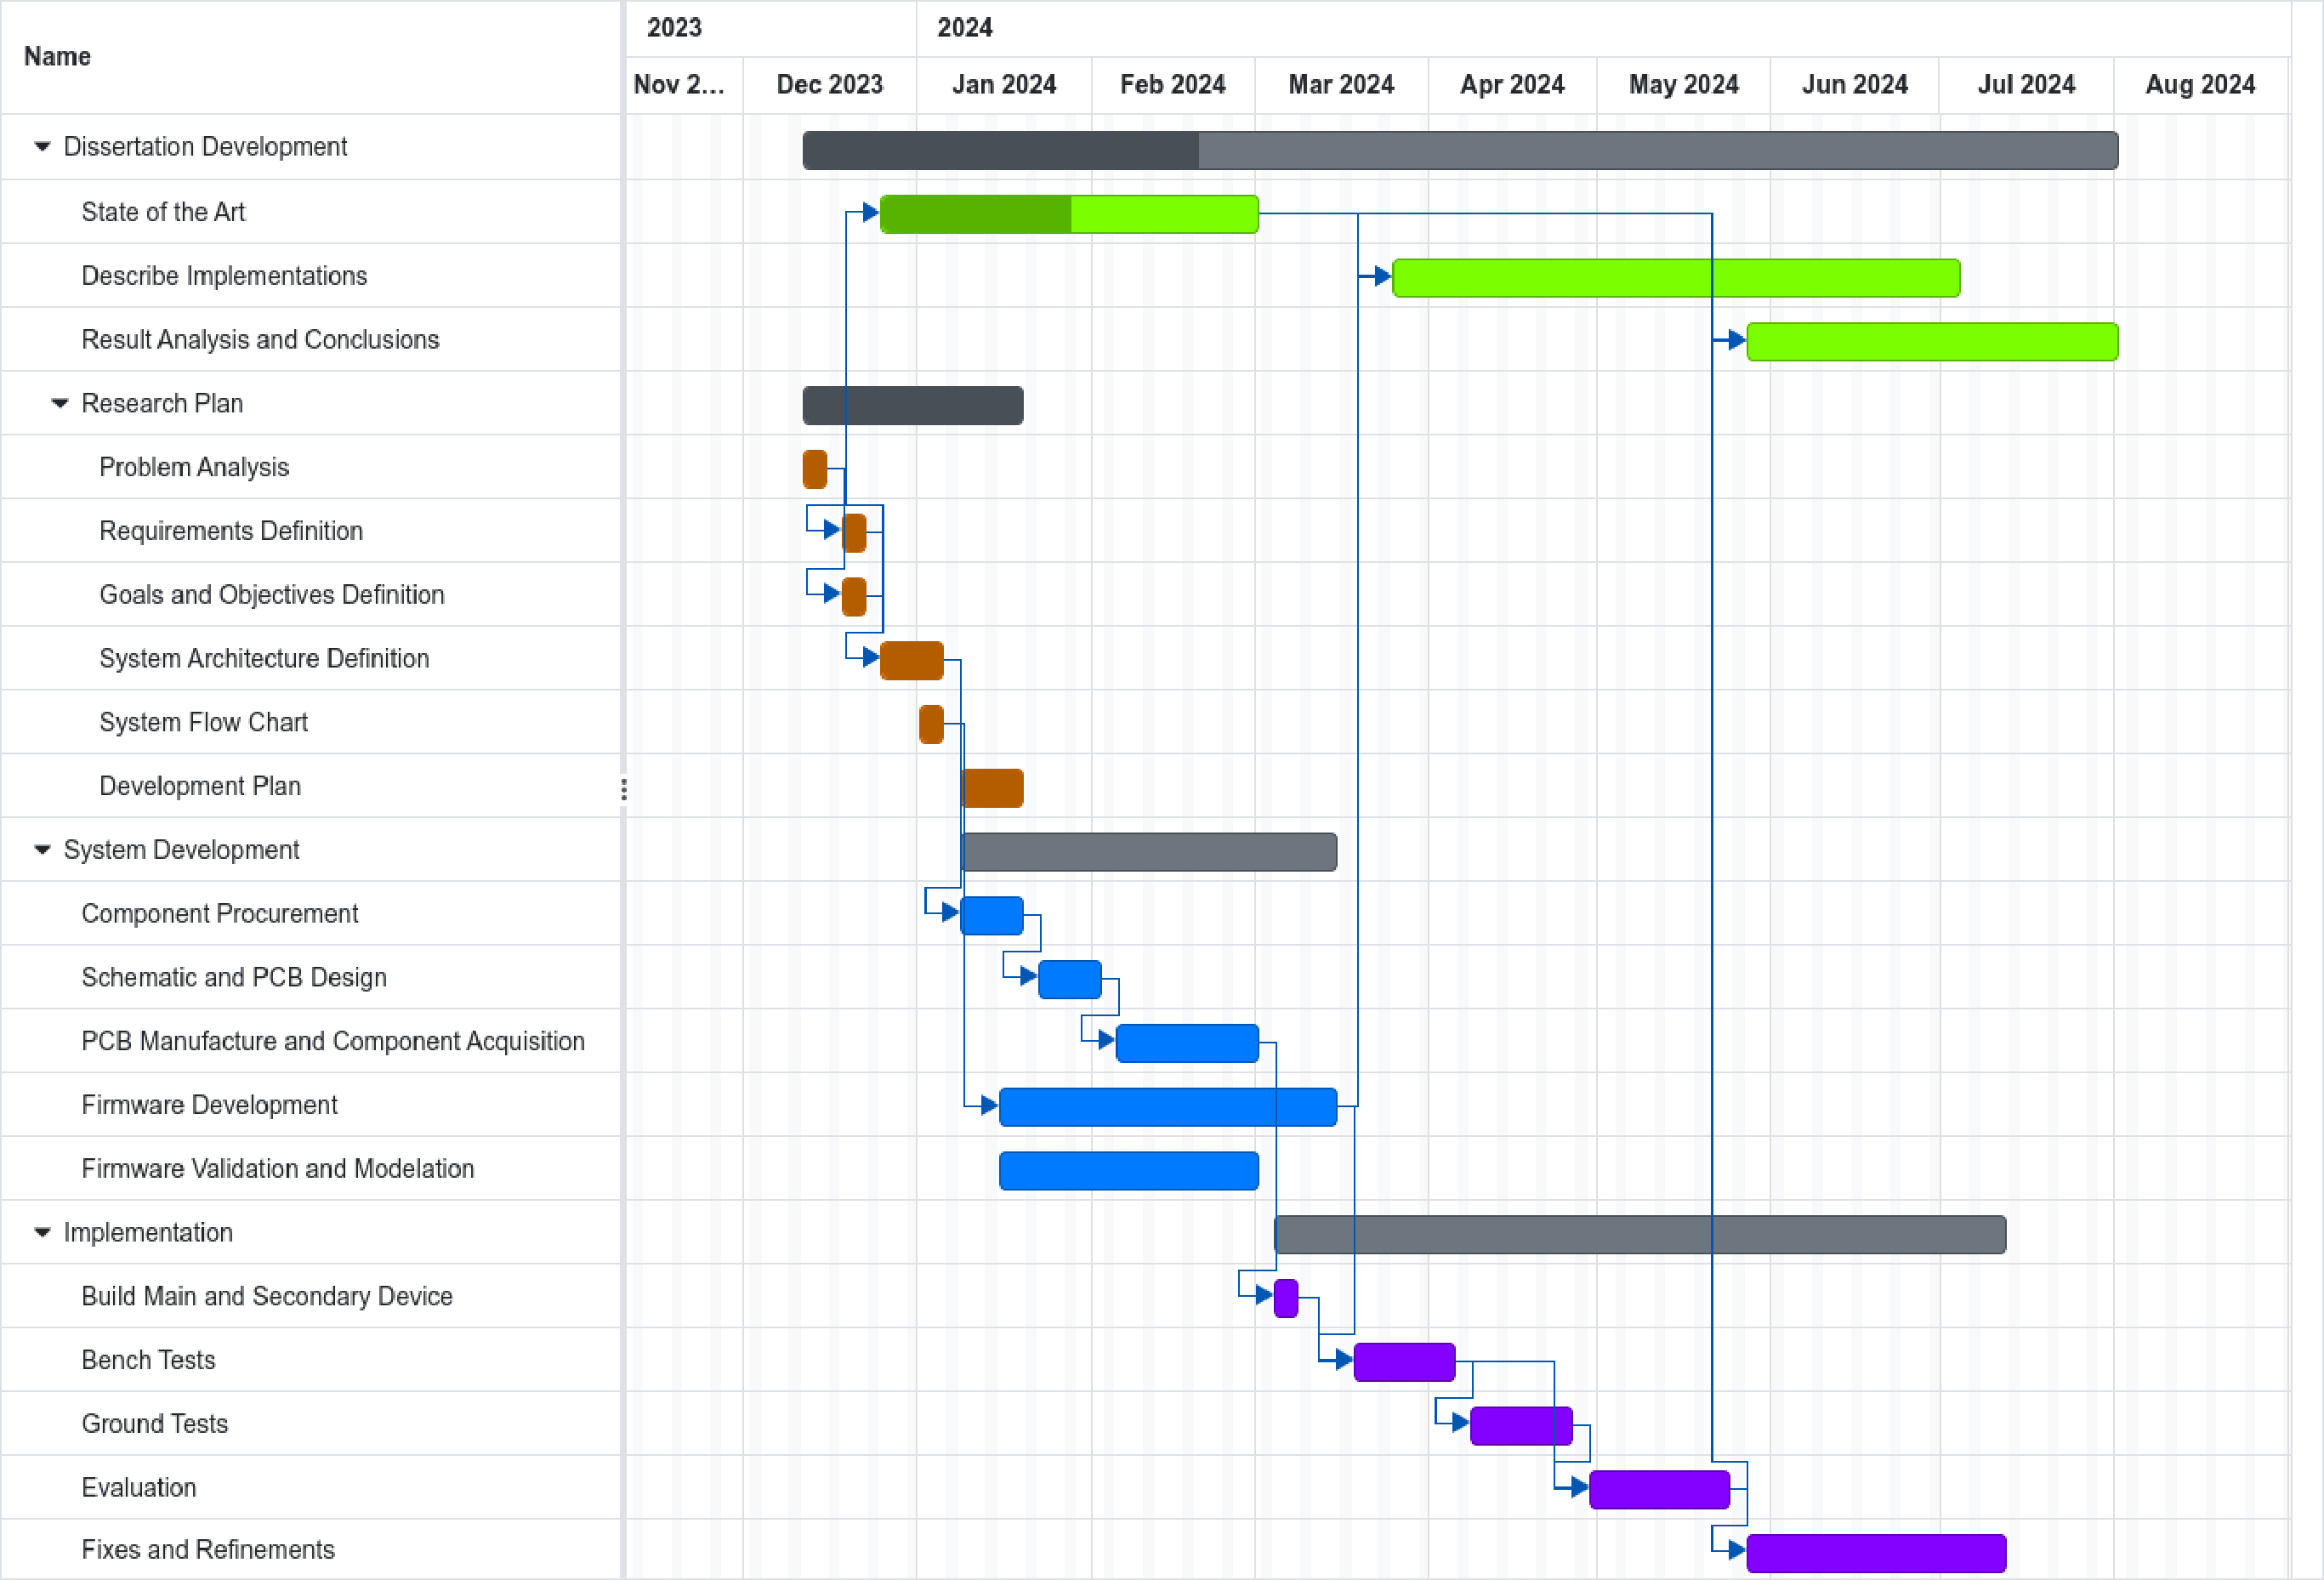
\includegraphics[width=\textwidth,keepaspectratio]{ch5/assets/gantt.pdf}
    \caption{Project timeline Gantt chart}
    \label{fig:gantt}
\end{figure}

The workload will be the following:

\begin{table}[H]
    \caption{Development Work Load}
    \label{tab:treatments}
    \centering
    \begin{tabular}{l l c}
        \toprule
        \tabhead{Type} & \tabhead{Name}           & \tabhead{Duration (days)} \\
        \midrule
        Main Task      & Dissertation Development & 170                       \\
        Sub Task       & Research Plan            & 30                        \\
        Main Task      & System Development       & 60                        \\
        Sub Task       & Hardware                 & 40                        \\
        Sub Task       & Firmware                 & 50                        \\
        Main Task      & Implementation           & 90                        \\
        Sub Task       & Tests                    & 30                        \\
        \bottomrule                                                           \\
    \end{tabular}
\end{table}

This timeline will help to ensure that all necessary activities are completed in the correct order and on time.

\section{Final Remarks}
Even if a detailed planning has been defined, unforeseen events may occur that delay the development of this Thesis.
The manufacture of the \glspl{PCB} and the purchase of the components are examples where, the delay in the arrival of the hardware will postpone the start of initial tests.

Even so, designing the development plan helped structure the main tasks needed to finish the development of this Thesis.
The comprehensive analysis and literature review, done in Dissertation Development phase, will set the foundation for defining system requirements, outlining objectives, and designing the system architecture.
This will be helpful during the selection of hardware components and firmware strategies, done in the System Development phase.

Both this phases lay the groundwork for the subsequent implementation of the developed solution, where the main prototype will be build and tested.
Through these evaluations, the developed system will be assessed against the goals and requirements described in previous chapters.

By analyzing the results it will be possible to determine if necessary refinements are needed.
